%-----------------------------------------------------------------------------%
\chapter{\babDua}
%-----------------------------------------------------------------------------%
Pada bab ini dijelaskan mengenai penelitian terkait dan berbagai dasar teori yang menunjang penelitian ini.

%-----------------------------------------------------------------------------%
\section{Penelitian Terkait}
%-----------------------------------------------------------------------------%

Sejak pertama kali diperkenalkan pada tahun 2007 \citep{banko2007open}, sudah ada beberapa penelitian mengenai \textit{open IE} untuk bahasa Inggris yang dipublikasikan. Sistem \textit{open IE} yang pertama diperkenalkan adalah \textsc{TextRunner} \citep{banko2007open}. Sistem ini kemudian dikembangkan oleh sistem-sistem dari penelitian berikutnya yaitu (secara berurutan) \textsc{ReVerb} \citep{fader2011identifying}, \textsc{R2A2} \citep{etzioni2011open} dan kemudian \textsc{Ollie} \citep{schmitz2012open}	. Selain itu, salah satu penelitian terbaru juga memperkenalkan sistem \textit{open IE} baru, \textsc{Stanford Open IE}, yang berhasil mengungguli kinerja \textsc{Ollie} dalam TAC-KBP 2013 \textit{Slot Filling task} \citep{angeli2015leveraging}.

Sistem \textit{open IE} yang pertama diperkenalkan adalah \textsc{TextRunner}. Sistem ini didesain untuk mengekstrak informasi secara efisien dari halaman-halaman \textit{web} di internet yang jumlahnya sangat besar dan memiliki domain yang berbeda-beda \citep{banko2007open}. Informasi yang diekstrak merupakan \textit{tuple} $t = (e_i, r_{i,j}, e_j)$ di mana $r_{i,j}$ adalah relasi antara entitas $e_i$ dan $e_j$ dalam sebuah kalimat. \textsc{TextRunner} terdiri dari tiga modul utama \citep{banko2007open} yaitu: (1) \textit{Self-Supervised Learner}, modul yang melatih sebuah \textit{naive bayes classifier} (NBC) untuk mengenali kandidat \textit{triple} yang valid tanpa memerlukan campur tangan manusia (\textit{self-supervised}), (2) \textit{Single-Pass Extractor}, modul yang mengekstrak sejumlah kandidat \textit{triple} dari setiap kalimat dan menyimpan kandidat yang dianggap valid oleh \textit{classifier}, dan (3) \textit{Redundancy-based Assessor}, modul yang menghitung probabilitas kemunculan \textit{triple} dalam satu dokumen. Sistem ini mampu mengekstrak informasi per kalimat dengan akurasi rata-rata 88\% dan mampu memproses 9 juta halaman \textit{web} dalam 68 \textit{CPU hours} \citep{banko2007open}.

\textsc{ReVerb} adalah sistem \textit{open IE} yang dikembangkan untuk memperbaiki dua masalah pada pendahulunya, \textsc{TextRunner}. Masalah yang ingin diselesaikan oleh \textsc{ReVerb} adalah inkoherensi hasil ekstraksi \textit{incoherent extractions} dan hasil ekstraksi yang tidak informatif \textit{uninformative extractions} \citep{fader2011identifying}. Untuk mengekstrak \textit{triple} $t = (e_i, r_{i,j}, e_j)$, sistem ini menggunakan dua algoritma utama, yaitu (1) \textit{Relation Extraction}, algoritma yang mengekstrak relasi $r_{i,j}$ menggunakan pembatasan sintaktik dan leksikal yang menyelesaikan dua masalah tersebut, dan (2) \textit{Argument Extraction}, algoritma yang mencari entitas $e_i$ dan $e_j$ yang dihubungkan oleh relasi $r_{i,j}$ menggunakan heuristik.  \textsc{ReVerb} menerima \textit{input} berupa kalimat yang telah dianotasi POS-nya \% potongan frase kata bendanya (NP \textit{chunk}) dan menghasilkan \textit{output} sejumlah \textit{triple}. Dari hasil pengujian yang dilakukan, \textsc{ReVerb} mencapai \textit{precision} dan \textit{recall} yang hampir dua kali lebih baik dari \textsc{TextRunner} \citep{fader2011identifying}.

Jika \textsc{ReVerb} memperbaiki masalah pada ekstraksi relasi, \textsc{R2A2} berfokus untuk memperbaiki ekstraksi argumen/entitas \citep{etzioni2011open}. Jika \textsc{ReVerb} hanya menggunakan aturan atau heuristik untuk mengekstraksi argumen \citep{fader2011identifying}, \textsc{R2A2} menggunakan modul berbasis \textit{machine learning}, \textsc{ArgLearner}. Modul ini menerima relasi dan kalimat sebagai \textit{input} dan mengembalikan dua buah argumen sebagai \textit{output}. Modul ini menggunakan tiga buah \textit{classifier} berbasiskan \textsc{REPTree} \citep{hall2009weka} dan \textit{sequence labeling} CRF \citep{mccallum2002mallet} untuk mengekstrak argumen dari kalimat melalui proses yang ditunjukkan pada Gambar \ref{fig_arglearner_architecture} \citep{etzioni2011open}.

\begin{figure}
\centering
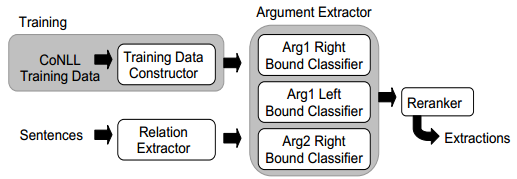
\includegraphics[scale=0.5]{../images/arglearner_architecture.png}
\caption{Proses pelatihan dan ekstraksi \textsc{ArgLearner}}
\label{fig_arglearner_architecture}
\end{figure}

Penelitian berikutnya memperkenalkan \textsc{Ollie} (\textit{Open Language Learning for Information Extraction}) \citep{schmitz2012open} yang menjadikan \textsc{ReVerb} sebagai salah satu modulnya. \textsc{Ollie} menggunakan \textsc{ReVerb} untuk mencari sejumlah (\textit{open pattern})/\textit{template} sebagai panduan untuk mengekstrak \textit{triple} dari kalimat. Perbedaan lain sistem ini dengan pendahulunya adalah relasi yang diekstrak tidak hanya dari kata kerja (\textit{verb}) tetapi bisa juga diekstrak secara implisit dari kata benda (\textit{noun}), kata sifat (\textit{adjective}) \citep{schmitz2012open}. Selain itu \textsc{Ollie} juga menambahkan modul untuk melakukan analisis dan penambahan informasi kontekstual pada hasil ekstraksi sehingga presisi lebih tinggi. Dua modul utama ini diajukan untuk memperbaiki kekurangan dari \textsc{ReVerb} yaitu pembatasan relasi hanya pada kata kerja (\textit{verb}) dan pengabaian konteks kalimat \citep{schmitz2012open}. Proses pelabelan (\textit{labeling}) data latih dan ekstraksi \textsc{Ollie} ditunjukkan pada Gambar \ref{fig_ollie_architecture}.

\begin{figure}
\centering
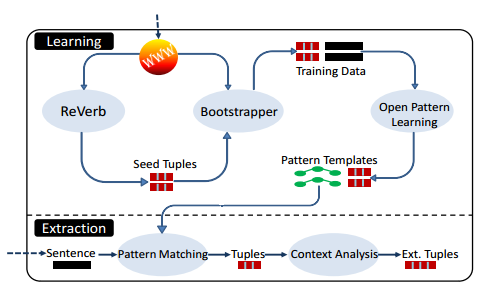
\includegraphics[scale=0.5]{../images/ollie_architecture.png}
\caption{Proses \textit{labeling} dan ekstraksi pada \textsc{Ollie}}
\label{fig_ollie_architecture}
\end{figure}

Salah satu riset terbaru memperkenalkan model sistem \textit{open IE} yang mengganti penggunaan banyak \textit{open pattern}/\textit{template} untuk mengekstrak \textit{triple} pada \textsc{Ollie} \citep{schmitz2012open} dengan hanya enam pola atomik (\textit{atomic patterns}) \citep{angeli2015leveraging}. Enam pola atomik itu digunakan untuk mengekstrak \textit{triple} dari klausa yang \textit{self-contained} dan \textit{maximally compact}. Modul ekstraktor \textit{inter-clauses}, yang menggunakan \textit{multinomial logistic regression classifier}, bertanggungjawab menghasilkan klausa yang \textit{self-contained} (independen secara sintaktik dan semantik), dan modul ekstraktor \textit{intra-clause}, yang menggunakan model \textit{natural logic} \citep{maccartney2007natural}, mengubahnya menjadi klausa yang \textit{maximally compact} (tidak mengandung kata redundan). Model sistem ini diimplementasikan dalam \textsc{Stanford Open IE}, yang merupakan bagian dari kakas NLP \textit{opensource}, \textit{Stanford Core NLP}\footnote{Stanford Core NLP \url{https://stanfordnlp.github.io/CoreNLP/}}.

%-----------------------------------------------------------------------------%
\section{\textit{Open Domain Information Extraction}}
%-----------------------------------------------------------------------------%

\textit{Open domain information extraction} (\textit{open IE}) adalah proses ekstraksi informasi dari dokumen dalam format \textit{triple} $(x, r, y)$ di mana $r$ adalah relasi antara dua buah argumen/entitas $x$ dan $y$ \citep{banko2007open, etzioni2011open}. Relasi pada \textit{triple} diambil dari kata kerja (\textit{verb}) \citep{banko2007open, fader2011identifying} (contoh: kalimat "\textit{Jakarta is the capital of Indonesia}" mengandung \textit{triple} ("Jakarta", "is the capital of", "Indonesia")) atau dari kata lain yang secara implisit merupakan kata kerja \citep{schmitz2012open} (contoh: "\textit{Indonesian President Joko Widodo was born in Surakarta}" mengandung \textit{triple} ("Joko Widodo", "be", "president")). Sedangkan argumen atau entitas yang diekstrak selalu merupakan frase (\textit{noun phrase}) seperti yang juga terlihat di contoh. Format \textit{triple} ini ternyata berlaku umum untuk semua dokumen yang berisi teks bahasa natural sehingga dapat diterapkan pada dokumen dari berbagai domain. Format \textit{triple} yang digunakan \textit{open IE} memiliki kemiripan dengan format yang lazim digunakan pada \textit{knowledge extraction} (KE), yaitu \textit{Resource Data Format} (RDF)\footnote{Resource Data Format W3C \url{https://www.w3.org/RDF/}} \citep{auer2007dbpedia, exner2014refractive}. Namun, perbedaannya adalah \textit{triple} pada \textit{open IE} umumnya tidak mengikuti seluruh spesifikasi RDF dan tidak memiliki himpunan ontologi tetap. Ringkasan perbandingan antara open IE dan KE ditunjukkan pada Tabel \ref{table_paradigm_comparison}. 

\begin{table}
	\centering
	\caption{Perbandingan antara \f{information extraction} tradisional (IE), \f{open domain extraction} (open IE) dan \f{knowledge extraction} (KE)}
	\label{table_paradigm_comparison}
	\begin{tabular}{l c c c}
		\hline 
		\textbf{Aspek} & \textbf{IE} & \textbf{Open IE} & \textbf{KE} \\ 
		\hline 
		\textbf{Domain} & Tertutup & Terbuka & Terbuka \\ 
		\textbf{Format} & Tergantung domain & Triples & RDF Triples \\ 
		\textbf{Ontologi} & Tidak tersedia & Opsional & Wajib \\ 
		\hline 
	\end{tabular} 
\end{table}

Meskipun menggunakan modul dan teknik yang berbeda-beda, model sistem \textit{open IE} umumnya menjalankan proses yang dapat dibagi menjadi tiga langkah/fase \citep{etzioni2011open}:

\begin{enumerate}
	\item Label (\textit{label}): membangun data latih untuk \textit{classifier} baik secara manual atau otomatis.
	\item Belajar (\textit{learn}): melatih \textit{classifier} untuk mengekstrak himpunan \textit{triple} dari kalimat menggunakan data dari fase Label.
	\item Ekstrak (\textit{extract}): mengekstrak himpunan \textit{triple} dari kalimat menggunakan \textit{classifier} yang telah dilatih pada fase Belajar
\end{enumerate}

Hasil ekstraksi \textit{open IE} berguna untuk berbagai \textit{task} seperti \textit{question answering}, \textit{slot filling} \citep{etzioni2011open}, \textit{common sense knowledge acquiring} \citep{singh2002open} dan \textit{information retrieval} \citep{etzioni2011search}. Selain itu, jika dilihat sebagai representasi teks atau dokumen, himpunan \textit{triple} dari \textit{open IE} dapat digunakan sebagai fitur untuk klasifikasi dan \textit{clustering} teks atau dokumen.

%-----------------------------------------------------------------------------%
\section{\textit{Natural Language Processing}}
%-----------------------------------------------------------------------------%

Pemrosesan bahasa natural atau \textit{natural language processing} (NLP) tidak bisa dipisahkan dari information extraction \citep{banko2007open,fader2011identifying,etzioni2011open,angeli2015leveraging}. Semua model sistem \textit{open IE} juga selalu membutuhkan informasi yang dihasilkan oleh \textit{task} NLP seperti \textit{part of speech tagging}, \textit{dependency parsing} dan \textit{named-entity recognition}. Informasi tersebut digunakan sebagai variabel dalam heuristik \textit{open IE} dan juga sebagai fitur untuk \textit{classifier}.

\subsection{\textit{Part of Speech Tagging}}

\textit{Part of speech} (POS) \textit{tagging} adalah \textit{task} NLP yang bertujuan menentukan \textit{POS tag} atau jenis setiap kata pada kalimat. Contoh \textit{POS tag} dasar adalah kata benda (\textit{noun}), kata kerja (\textit{verb}), kata sifat (\textit{adjective}) dst. Gambar \ref{fig_example_pos_tagging} menunjukkan contoh \textit{POS tagging} terhadap kalimat sederhana. \textit{POS tag} dapat digunakan juga oleh \textit{NLP task} yang lain seperti \textit{dependency parsing} dan \textit{named-entity recognition}.

\begin{figure}
	\begin{mdframed}
		\textbf{Input}: "Ibu pergi ke pasar." \\		
		\textbf{Output}: (Ibu, \textit{noun}) (pergi, \textit{verb}) (ke, \textit{preposition}) (pasar, \textit{noun}) (., \textit{punctuation})
	\end{mdframed}
	\caption{Contoh \textit{input} dan \textit{output} \textit{POS tagging}}
	\label{fig_example_pos_tagging}
\end{figure}


\subsection{\textit{Dependency Parsing}}

\lipsum[6]

\subsection{\textit{Named-Entity Recognition}}

\lipsum[5]

\subsection{CONLL-U}

\lipsum[4]

%-----------------------------------------------------------------------------%
\section{\textit{Supervised Learning}}
%-----------------------------------------------------------------------------%

\lipsum[3]

\subsection{\textit{Logistic Regression}}

\lipsum[4]

\subsection{\textit{Support Vector Machine}}

\lipsum[5]

\subsection{\textit{Multi-Layer Perceptron}}

\lipsum[6]

\subsection{\textit{Random Forest}}

\lipsum[7]

\subsection{\textit{Cross Validation}}

\lipsum[8]
